\documentclass[a4paper, 12pt]{article}
\usepackage[swedish]{babel}
\usepackage[utf8]{inputenc}
\usepackage{verbatim}
\usepackage{fancyhdr}
\usepackage{graphicx}
\usepackage{parskip}
% Include pdf with multiple pages ex \includepdf[pages=-, nup=2x2]{filename.pdf}
\usepackage[final]{pdfpages}
% Place figures where they should be
\usepackage{float}

% vars
\def\title{Plugin 1.2}
\def\preTitle{Laboration 1}
\def\kurs{Applikationsprogrammering i Java, HT-08}

\def\namn{Anton Johansson}
\def\mail{dit06ajn@cs.umu.se}
 \def\pathtocode{$\sim$dit06ajn/edu/apjava/lab1}

\def\handledareEtt{Johan Eliasson johane@cs.umu.se}
\def\inst{datavetenskap}
\def\dokumentTyp{Laborationsrapport}

\begin{document}
\begin{titlepage}
  \thispagestyle{empty}
  \begin{small}
    \begin{tabular}{@{}p{\textwidth}@{}}
      UMEÅ UNIVERSITET \hfill \today \\
      Institutionen för \inst \\
      \dokumentTyp \\
    \end{tabular}
  \end{small}
  \vspace{10mm}
  \begin{center}
    \LARGE{\preTitle} \\
    \huge{\textbf{\kurs}} \\
    \vspace{10mm}
    \LARGE{\title} \\
    \vspace{15mm}
    \begin{large}
        \namn, \mail \\
        \pathtocode
    \end{large}
    \vfill
    \large{\textbf{Handledare}}\\
    \mbox{\large{\handledareEtt}}
  \end{center}
\end{titlepage}

\pagestyle{fancy}
\rhead{\today}
\lhead{\namn, \mail}
\chead{}
\lfoot{}
\cfoot{}
\rfoot{}

\tableofcontents
\newpage

\rfoot{\thepage}
\pagenumbering{arabic}

\section{Problemspecifikation}
% Beskriv med egna ord vad uppgiften gick ut på. Är det någonting som
% varit oklart och ni gjort egna tolkningar så beskriv dessa.
Denna laboration gick ut på att skriva ett Javaprogram som använder
sig av Javas paket \textit{java.lang.reflect}. Paketet har funktioner
som gör det möjligt att inspektera, instansera, modifiera och exekvera
objekt och klasser medan ett program körs.

Till detta program skulle ett grafiskt gränssnitt skrivas. Från det
grafiska gränssnittet skulle metoder kunna exekveras och eventuell
utdata skulle skrivas ut i ett textfält.

Problemspecifikation finns i original på:\\
\verb!http://www.cs.umu.se/kurser/5DV085/HT08/labbar/lab1.html!

\section{Användarhandledning}
% Förklara var programmet och källkoden ligger samt hur man startar,
% kompilerar och använder det.
Programmet ligger i katalogen: \pathtocode

Från denna katalog kompileras programmet med kommandot:

\verb!salt:~/edu/apjava/lab1> ant!

Källkoden ligger i underkatalogen \verb!src!.

Programmet tar vid start emot ett argument, detta ska vara namnet på
en klass som implementerar gränssnittet Plugable (se bilaga
\ref{plugable.java}), har en konstruktor utan parametrar och finns
tillgängligt i aktuell classpath. För att köra programmet med klassen
\textit{Calc}:

\verb!salt:~/edu/apjava/lab1> java -cp bin/prod/ MyToolbox Calc!

Detta resulterar i det grafiska gränssnitt som visas i figur
\ref{fig:gui}.

\begin{figure}[H]
  \begin{center}
    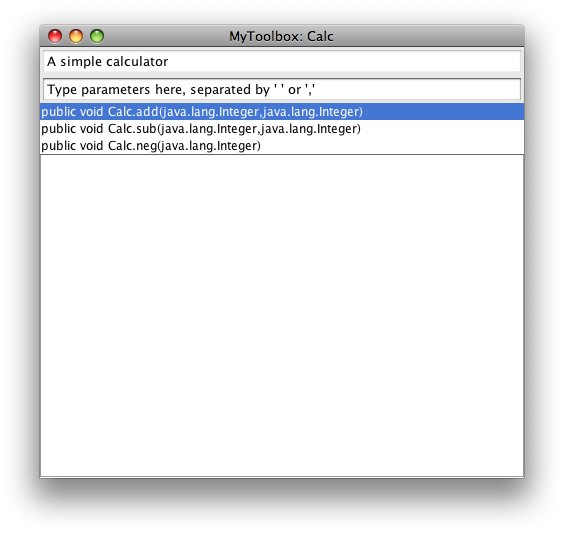
\includegraphics[width=110mm]{images/gui-out.png}
    \caption{GUI}
    \label{fig:gui}
  \end{center}
\end{figure}

I figur \ref{fig:gui} visar första fältet beskrivningen för klassen
\textit{Calc}. I nästa fält kan användaren ange parametrar som kan
behövas för att exekvera klassens metoder. I listan under vissas alla
metoder som är direkt deklarerade i klassen.

För att köra en metod fyller användaren i nödvändiga parametrar,
separerade av mellanslags- eller komma-tecken, i parameterfältet och
trycker \verb!ENTER!, då körs markerad metod i
metodlistan. Alternativt kan användaren dubbelklicka på en metod, då
körs denna metod med de parametrar som finns ifyllda i
parameterfältet.

\section{Systembeskrivning}
% Beskriv översiktligt hur programmet är uppbyggt och hur det löser
% problemet.
Programmet består huvudsakligen av två klasser, \textit{MyToolbox} och
\textit{ClassHandler}. Klassen \textit{MyToolbox} startar programmet
och har ansvar för att rita det grafiska gräns\-snittet, klassen
kontrollerar även indata och utdata till och från använd\-aren. I en
''Model-View-Controller''-design skulle klassen \textit{MyToolbox}
motsvara ''View-Controller''-delen. I samma modell motsvarar klassen
\textit{ClassHandler} ''Model''-delen, det vill säga det är i
\textit{ClassHandler} som programmet har sin grundfunktionalitet och
data. Figur \ref{fig:class} visar ett klassdiagram av programmet.

\begin{figure}[H]
  \begin{center}
    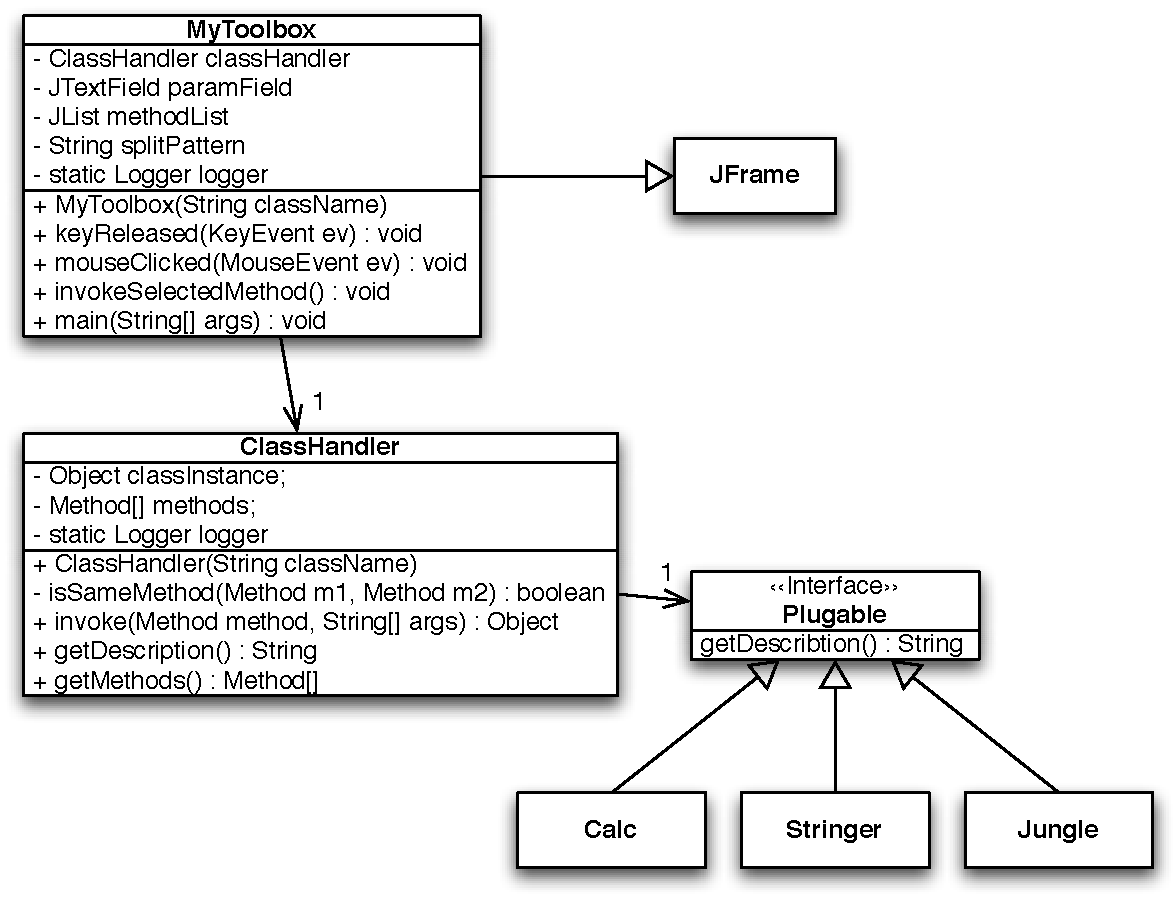
\includegraphics[width=130mm]{images/class.pdf}
    \caption{Klassdiagram}
    \label{fig:class}
  \end{center}
\end{figure}

\subsection{API-dokumentation}
API-dokumentation för programmet finns att läsa på:\\
\verb!http://www.cs.umu.se/~dit06ajn/apjava/lab1/!

\subsection{MyToolbox.java}
Klassen \textit{MyToolbox} ritar upp det grafiska gränssnittet genom
att ärva från klassen \textit{JFrame}. I klassens konstruktor skapas
en instans av klassen \textit{ClassHandler} och alla element som finns
i gränssnittet skapas och läggs in i paneler av typ
\textit{JPanel}. Lyssnare, Javas \textit{KeyAdapter} respektive
\textit{MouseAdapter}, kopplas till det grafiska fältet som tar emot
parametrar och listan som innehåller metoder. Dessa lyssnare har
metoder som reagerar på musklick och tangentbordstryck, när något av
detta händer så kommer vald metod att exekveras genom ett anrop till
klassen \textit{ClassHandler}.

I \textit{main}-metoden som används för att starta programmet fångas
eventuella undantag som hindrar fortsatt exekvering av
programmet. Exempel på sådana undantag är om argumentet som skickas
med till MyToolbox inte är namnet på en klass som återfinns vid
körning, om denna klass inte implementerar \textit{Plugable} eller om
klassen inte har en standardkonstruktor utan parametrar.

All utdata från eventuella metodkörningar omdirigeras till det
grafiska gräns\-snittets textfält. Detta görs med hjälp av de givna
klasserna \textit{TextAreaWriter} och \textit{WriterOutputStream}, se
bilaga \ref{taw} och \ref{wos}. Detta gäller alla utskrifter som görs
via metoderna i \textit{System.out}. Eventuella värden som returneras
från metodanrop skrivs enligt specifikationen inte ut.

Källkod finns i bilaga \ref{mytoolbox.java}.

\subsection{ClassHandler.java}
Klassen \textit{ClassHandler} tar emot en textsträng i sin
konstruktor. Denna textsträng ska vara namnet på en klass som
implementerar gränssnittet Plugable och finns i aktuell classpath när
programmet körs. En ny instans av klassen med det medskickade namnet
skapas med hjälp av metoderna \textit{Class.forName()} och
\textit{Class.newInstance()} i Javas paket \textit{java.lang.reflect}.

Alla metoder deklarerade i den laddade klassen, som inte är
implementationer från gränssnittet \textit{Plugable}, sparas undan i ett
fält \textit{methods}. Metoder för att hämta och köra dessa metoder är
implementerade. Ytterligare finns en metod för att hämta en kort
beskrivning av den laddade klassen, denna metod anropar den laddade
klassens metod \textit{getDescription()} som är ett krav från
gränssnittet \textit{Plugable}.

Källkod finns i bilaga \ref{classhandler.java}.

\subsection{Plugable.java}
Gränssnittet \textit{Plugable} garanterar att klasserna som laddas in i
\textit{ClassHandler} har en metod \textit{getDescription()} som
returnerar en kort textsträng med en beskrivning av den laddade
klassens funktionalitet.

\section{Begränsningar}
% Vilka problem och begränsningar har din lösning av uppgiften? Hur
% skulle de kunna rättas till?

Eftersom man vid start av programmet skickar in klassnamnet på klassen
som ska laddas när man startar programmet från terminalen sköts många
undantag, som inte går att korrigeras, i main metoden. Det erbjuds
ingen möjlighet att ändra eller korrigera klass i det grafiska
gränssnittet, därför stängs programmet ner vid felaktig eller icke
existerande klass. Om det grafiska gränssnittet kunnat hantera detta
hade denna hantering flyttats.

Kravet på att klassen som laddas in i programmet ska implementera
gräns\-snittet \textit{Plugable} hade inte behövt vara så hårt, man
skulle lika gärna kunna ladda in vilken klass som helst, skillnaden
hade blivit att man inte fått någon kort beskrivning av klassen. Detta
hade kunnat fixas genom att spara undan instansen av den laddade
klassen av typen \textit{Object} istället för \textit{Plugable}, vid
körning av metoden \textit{getDescription()} hade det då behövts en
kontroll för att se om objektet är en instans av \textit{Plugable}.

Tolkningen av indatan som fås ur fältet som tar emot parametrar från
anv\-ändaren hade kunnat göras mer avancerat. I nuläget delas
parametrarna upp med avseende på mellanslags-tecken och komma-tecken,
det hade varit önskvärt att även kunna ange en textsträng inom
situationstecken \verb!"! för att ange en parameter som innehåller en
textsträng som internt kan innehålla mellanslags-tecken och
komma-tecken.

% TODO - Vad händer om man laddar en klass utan metoder, inga
% relevanta felmeddelanden och det kan bli nullpointer

\section{Reflektioner}
% Var det något som var speciellt krångligt? Vilka problem uppstod och
% hur löste ni dem? Allmänna synpunkter. Hur skulle man kunna använda
% dessa metoder i andra mer omfattande system?

Dokumentation av källkoden med hjälp av \textit{Javadoc}, resulterade
i att samma dokumentation var nödvändig på flera ställen. Detta gäller
specifikt dokumentationen av undantagen som kastas vidare från klassen
\textit{ClassHandler} till \textit{MyToolbox} och internt i
\textit{MyToolbox} från konstruktorn till main-metoden.

Metoderna i \textit{java.lang.reflect} verkar högst användbara
speciellt när det gäller att skapa utvecklingsverktyg för Java. Till
exempel skulle metoderna i \textit{java.lang.Class} kunna användas för
att automatiskt generera UML-diagram för ett program.

\section{Testkörningar}
% Noggranna testkörningar där man ser att programmet fungerar som det ska.
Nedan följer ett antal testkörningar som visar på olika scenarion vid
exekvering av programmet.

\subsection{Start av program}
Nedan följer spårutskrifter som visar på vad som händer vid start av
program där klassen som laddas inte följer specificerade
krav. Klasserna \textit{CalcNoEmtpyConstr} och
\textit{CalcNotPlugable} kan ses i bilage \ref{cnec} coh
\ref{cnp}. Klassen \textit{NonExistentClass} finns inte.

\begin{verbatim}
bash-3.2$ java -cp bin/prod MyToolbox CalcNoEmtpyConstr
Could not create an instance of this class. One empty \
constructor required
bash-3.2$ java -cp bin/prod MyToolbox CalcNotPlugable
Class must implement interface Plugable
bash-3.2$ java -cp bin/prod MyToolbox NonExistentClass
Class not found
\end{verbatim}

\subsection{Metodanrop}
Bild i figur \ref{fig:test1-out} visar på metodanrop med parametrarna
\verb!1 2!, det vill säga metoderna \textit{Calc.add(1, 2)},
\textit{Calc.sub(1, 2)} och sist \textit{Calc.neg(1 2)} körs. Utdata
blir:

\begin{verbatim}
3
-1
1 parameter(s) is required to to execute this method
\end{verbatim}

Om användaren inte har någon metod markerad när \verb!ENTER! trycks i
parameterfältet fås utdata ''\verb!No method is selected!'', detta sker
bara om användaren explicit avmarkerar den markerade metoden. Som
standard är alltid första metoden i listan markerad.

\begin{figure}[H]
  \begin{center}
    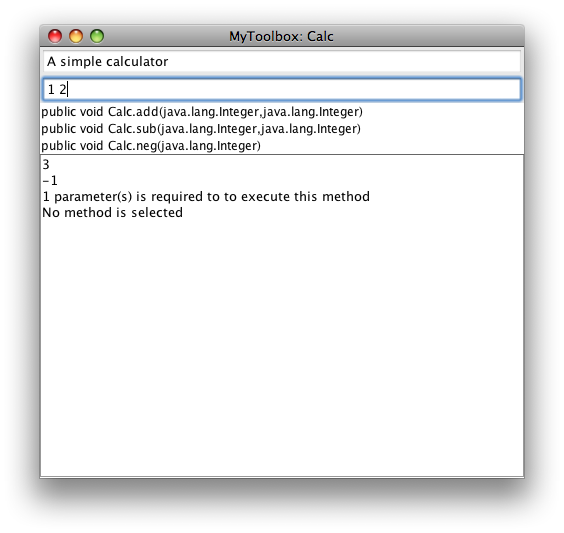
\includegraphics[width=110mm]{images/test1-out.png}
    \caption{Metodanrop}
    \label{fig:test1-out}
  \end{center}
\end{figure}

\section{Diskussion}
% Hur fungerade det att följa en kodkonvention? Vilka var fördelarna
% respektive nackdelarna?

Det fungerade bra att följa Javas kodkonvention, se:

\verb!http://java.sun.com/docs/codeconv/index.html!

Fördelen med att följa en kodkonvention är att om många följer samma
konvention blir koden mer lättläst. Att vara konsekvent när det gäller
kodstil är alltid positivt, även om det inte alltid är helt lätt att
till hundra procent följa en konvention, vilket bland annat visas av
att det i exemplen från Javas kodkonvention förekommer avvikelser från
själva kodkonventionen.

Konventionen att kommentera och dokumentera källkoden direkt med
\textit{Javadoc} underlättar otroligt mycket. Hade det inte varit för
Javas egen utförliga API-dokumentation hade mycket av denna laboration
varit  avsevärt krång\-ligare att utföra.

\newpage
\appendix
\pagenumbering{arabic}
\section{Källkod}
% Källkoden ska finnas tillgänglig i er hemkatalog
% ~/edu/apjava/lab1/. Bifoga även utskriven källkod.
Härefter följer utskrifter från källkoden till denna laboration.

\subsection{MyToolbox.java}\label{mytoolbox.java}
\begin{footnotesize}
\verbatiminput{../src/MyToolbox.java}
\end{footnotesize}
\newpage

\subsection{ClassHandler.java}\label{classhandler.java}
\begin{footnotesize}
\verbatiminput{../src/ClassHandler.java}
\end{footnotesize}
\newpage

\subsection{Plugable.java}\label{plugable.java}
\begin{footnotesize}
\verbatiminput{../src/Plugable.java}
\end{footnotesize}
\newpage

\subsection{Jungle.java}
\begin{footnotesize}
\verbatiminput{../src/Jungle.java}
\end{footnotesize}
\newpage

\subsection{CalcNoEmtpyConstr.java}\label{cnec}
\begin{footnotesize}
\verbatiminput{../src/CalcNoEmtpyConstr.java}
\end{footnotesize}
\newpage

\subsection{CalcNotPlugable.java}\label{cnp}
\begin{footnotesize}
\verbatiminput{../src/CalcNotPlugable.java}
\end{footnotesize}
\newpage

\subsection{TextAreaWriter.java}\label{taw}
\begin{footnotesize}
\verbatiminput{../src/TextAreaWriter.java}
\end{footnotesize}
\newpage

\subsection{WriterOutputStream.java}\label{wos}
\begin{footnotesize}
\verbatiminput{../src/WriterOutputStream.java}
\end{footnotesize}
\end{document}